\documentclass[11pt, letterpaper, titlepage]{article}
\usepackage[utf8]{inputenc}
\usepackage[export]{adjustbox}
\usepackage{geometry}
 \geometry{
 a4paper,
 total={168mm,257mm},
 left=20mm,
 top=15mm,
 includefoot,includehead
 }
\usepackage[backend=biber, style=authoryear, giveninits=true, maxbibnames=25, uniquename=init, maxcitenames=2, hyperref=true, dashed=false]{biblatex}			% Benutze Biber/BibLaTeX zum Zitieren
\addbibresource{report_short.bib}
\renewcommand{\cite}{\parencite}
\usepackage{caption}
\usepackage{subcaption}
\usepackage{graphicx}
\usepackage{svg}
\usepackage{placeins}
\usepackage[hidelinks]{hyperref}
\usepackage{amsmath}
\usepackage[headsepline]{scrlayer-scrpage}
\usepackage{acronym}

\clearpairofpagestyles %Seitenzahl nicht in der Kopfzeile

\title{MeetEU Project - Team Heidelberg - Team 1 -- \\ Identification and Enhancement of novel Sars-CoV-2 NSP13 Helicase Inhibitors}
\author{Linda Blaier, Paul Brunner, Selina Ernst, Valerie Segatz, and Chlo\'{e} Weiler}
\date{February 2024}

\begin{document}

\maketitle

\ihead{\headmark}
\automark{section}  %Kopfzeile gleich dem Sektiontitel
\cfoot{\pagemark}   %\ofood Seitenzahl rechts

\section{Workflow}

\begin{figure}[h]
  \centering
  %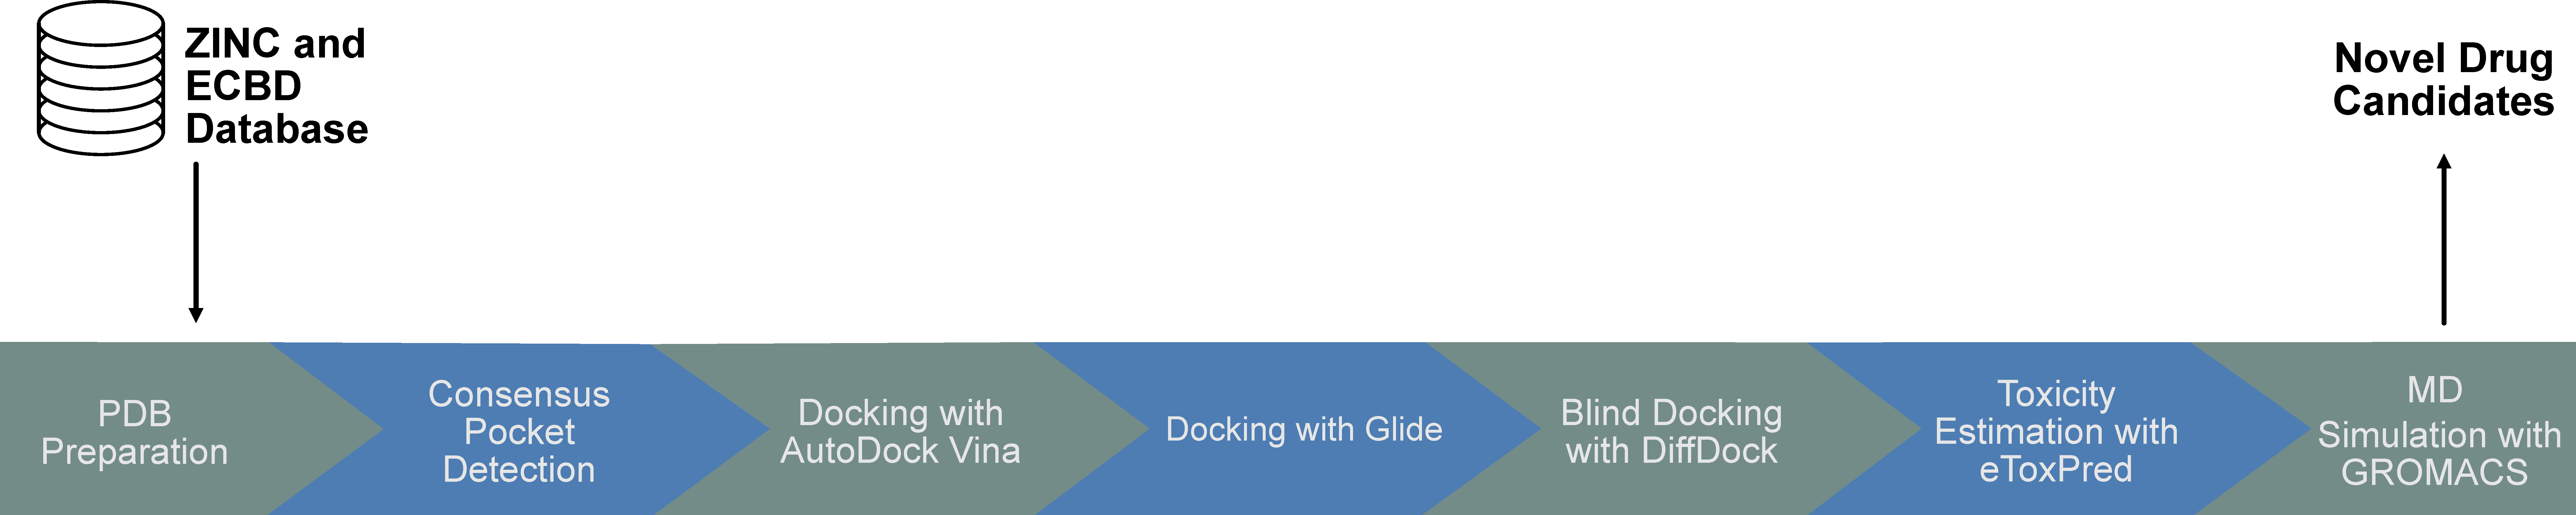
\includegraphics[width=\textwidth]{Workflow_MeetEU.pdf}
  \caption*{\textbf{Workflow for the discovery of NSP13 helicase inhibitors.}}
  \label{workflow}
\end{figure}

\setcounter{figure}{0}
\renewcommand{\thefigure}{\arabic{figure}}


\section{Material and Methods}
%\subsection{Datasets from ZINC20 and ECBD}
A total of 1616 FDA-approved drugs in \textit{.sdf} format from the ZINC database \cite{Irwin.2020} and 5016 files from the ECBD pilot library were downloaded.
%\subsection{Receptor and Ligand Preparation}
Three protein structures of NSP13 (PDB codes: 6ZSL, 5RME, and 5RM2) were aquired from RCSB PDB. For identification of the optimal consensus pocket. we used all these structures and applied multiple approaches (\textit{Fpocket} \cite{package_Fpocket}, \textit{PrankWeb 3} \cite{package_P2Rank,package_PrankWeb,package_PrankWeb3}, and \textit{FTMap} \cite{package_FTMAP}). For further experiments, the docking box was set to an cubic with an edge length of 30 \AA. Molecular Docking was performed using the A chain of 6ZSL file which was prepared using \textit{PDBFixer} \cite{Eastman_2017}. Ligands .sdf were converted into .pdbqts using \textit{OpenBabel} \cite{OpenBabel}. Molecular docking of the ligands was performed using \textit{AutoDock Vina} \cite{Trott.2010} and \textit{Glide} \cite{Friesner2004}. The docking results were then validated through blind docking with \textit{DiffDock} \cite{Corso.2022}. Toxicity and synthetic accessibility of the Top 100 scorers from \textit{AutoDock Vina} were predicted using \textit{eToxPred} \cite{pu2019toxpred}.
%\subsection{Molecular Dynamics Simulation}
In order to validate the binding of the top scorer, molecular dynamics simulation was performed using \textit{Gromacs} \cite{packageGROMACS}.\\

\section{Results}
The location of our consensus pocket was found within the ATP binding site, between the RecA-like domains A1 and A2. The molecular docking with \textit{AutoDock Vina} indentified 100 top scorers, which were ranked by their binding affinity, ranging from -10.3 to -8.8 $\frac{kcal}{mol}$. Passing these top 100 compounds through \textit{Glide} returned the following top three compounds: ZINC000096077632 (popular name: Angiotensin 1-7), ZINC000008101127 and ZINC000035880991. While they exhibit good binding affinities, they still do not bind as well as ATP.\textit{DiffDock} did not predict our Top 1 Glide scorer within our binding box, however  molecular dynamics simulation suggested a stable bond between the ligand and the helicase in our consensus pocket, as the ligand stayed inside of the pocket through the whole simulation. Multiple hydrogen bonds can be observed at the end of the 100 ns simulation, which almost all were found by \textit{Glide} before. The estimation of toxicity and synthetic accessibility using \textit{eToxPred} showed that only one out of out top 100 compounds is suggested to be toxic. Furthermore, most of the compounds seem to be very accessible in their synthesis.\\ 

\FloatBarrier

\section{Discussion and Outlook}
Throughout this project we were able to demonstrate a viable pipeline to screen and investigate possible ligands for biological targets. Analysis of the used data bases revealed a list of potential inhibitors of the NSP 13 helicase and thus therapeutics. The top scoring ligand, Angiotensin 1-7, has already been described in the context of treatment of Covid-19 \cite{angio}. 


\pagebreak
\FloatBarrier
\renewcommand{\bibname}{References}  % damit Literatuverzeicnis mit "References" betitelt
\printbibliography



\end{document}
